% !TEX root = ../thesis-main.tex

\chapter{Outlook}
\label{C:outlook}

\begin{epigraph}
  It was evening all afternoon. \\
  It was snowing \\
  And it was going to snow. \\
  The blackbird sat \\
  In the cedar-limbs.
\end{epigraph}

In this thesis we explored many ways in which algebraic invariants for filtered spaces can be defined and computed. There is still much more to investigate, and we present some ongoing work. We freely use the notations and results of the included papers.

\section{Replacing kernels with cokernels}

Following discussions with Andrea Guidolin and Bjørnar Gullikstad Hem.

Recall from Paper \ref{PC:CGRST2024} that for the lower hook parameterization, we have $\Nat(\cc{T}(a, b), F) = \ker F(a \leq b)$. Denote by $\pi_1$ and $\pi_2$ the two projections $\Omega(I) \to I$. We get two functors $F \pi_1$ and $F \pi_2$ and a natural morphism $\alpha \colon F \pi_1 \to F \pi_2$ between them. The following long exact sequence in $\Fun(\Omega(I), \Vect)$
\[
  0 \to \ker F(- \leq -) \hookrightarrow F \pi_1 \xrightarrow{\alpha} F \pi_2 \twoheadrightarrow \coker F(- \leq -) \to 0
\]
induces the following short exact sequences:
\begin{gather*}
  0 \to \ker F(- \leq -) \hookrightarrow F \pi_1 \twoheadrightarrow \im \alpha \to 0, \\
  0 \to \im \alpha \hookrightarrow F \pi_2 \twoheadrightarrow \coker F(- \leq -) \to 0.
\end{gather*}

Now suppose that $I$ is a two-dimensional grid (this should generalize to higher dimensions). Let $(a \leq b)$ be an element of $\Omega(I)$ with at least $3$ parents: in other words, $a$ and $b$ share at most one coordinate (of the two). Then we can show that the Koszul complex of $F \pi_i$, for $i = 1, 2$, is a product of chain complexes, one of which is contractible, and thus the homology of the Koszul complex is $0$ in all degrees.

Short exact sequences induce long exact sequences in homology: using the $0$'s of the homology of $F \pi_i$, we get the following isomorphisms for all $d \geq 0$:
\[
  H_d(\ker F(- \leq -)) \cong H_{d + 1}(\im \alpha) \cong H_{d + 2}(\coker F(- \leq -))
\]
Therefore, in order to compute Betti diagrams relative to lower hooks, we can study the Koszul complex of $\coker F(- \leq -)$ instead of $\ker F(- \leq -)$. This has some theoretical computational advantages: in order to compute a kernel basis, we need $O(n^2)$ space, where $n$ is the ambient dimension. In order to compute a cokernel basis, we only need $O(n)$ space, because we can choose representatives in the quotient space that correspond to canonical basis elements.

I have implemented this cokernel approach in Python, to middling success: see \cref{F:coker-results} for some experimental results. In \cref{F:cokerhooks}, we observe the exact same relative Betti diagrams as in \cref{F:lowerhooks}, except translated by $2$ degrees. In \cref{F:dev-time}, we see that the time required to compute relative Betti diagrams does not change when switching to cokernels, and in fact worsens a little bit. This may be explained by the fact that the cokernel complexes are larger in general than the corresponding kernel complexes: see \cref{F:dev-hist}. It is unclear where this is by nature or by the synthetic way in which they were constructed for this experiment, and this is worth exploring further.

\begin{figure}[t]
  \begin{subfigure}{\textwidth}
    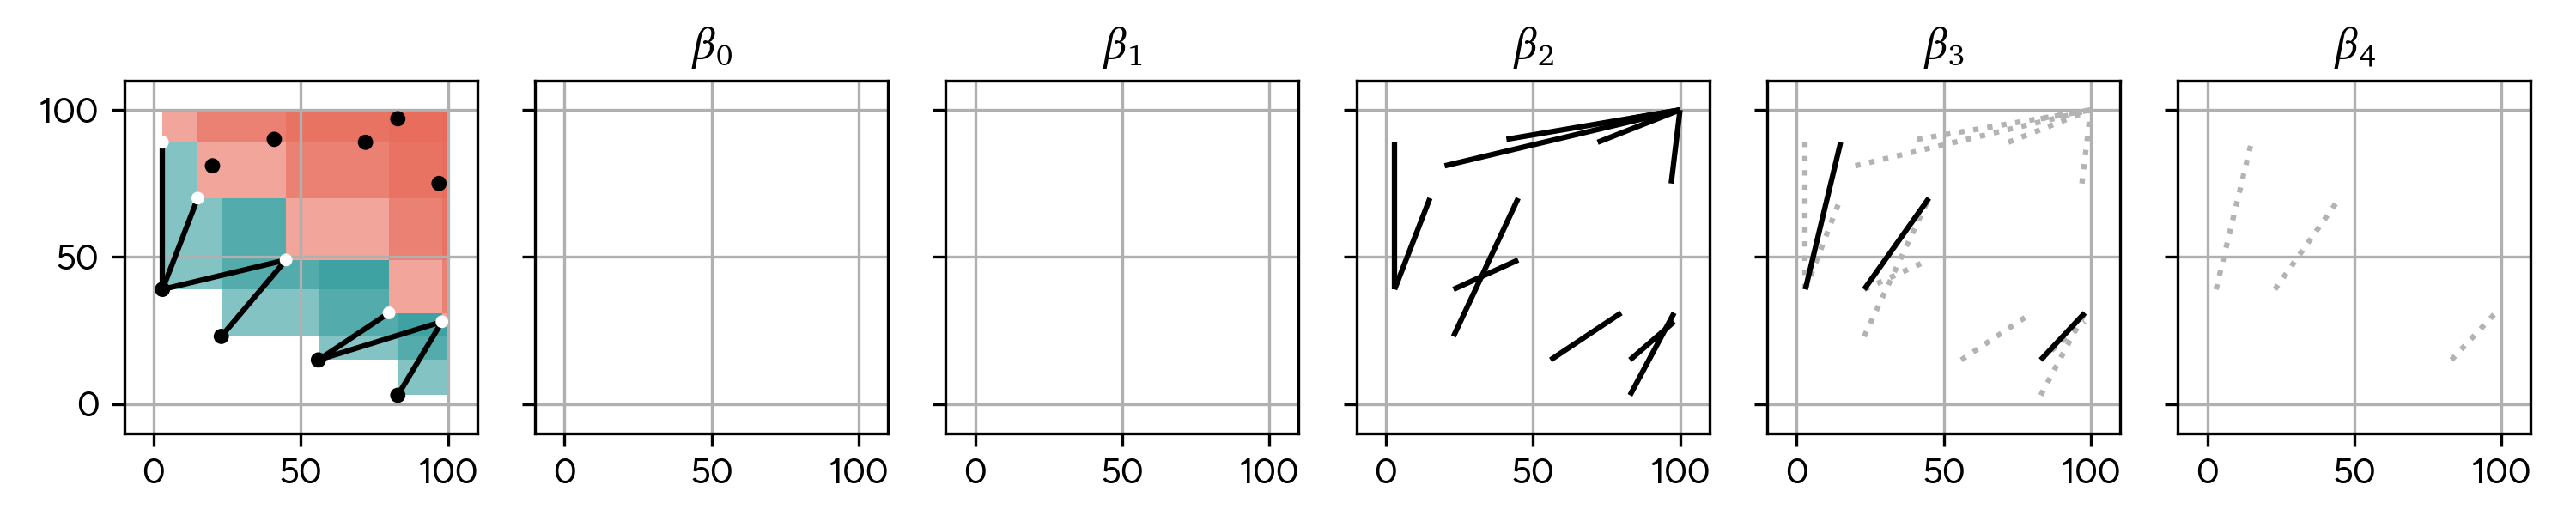
\includegraphics[width=\textwidth]{figs/cokerhooks.png}
    \caption{Result of computing the homology of the cokernel complex; compare with \cref{F:lowerhooks}.}
    \label{F:cokerhooks}
  \end{subfigure}
  \\
  \begin{subfigure}{.4\textwidth}
    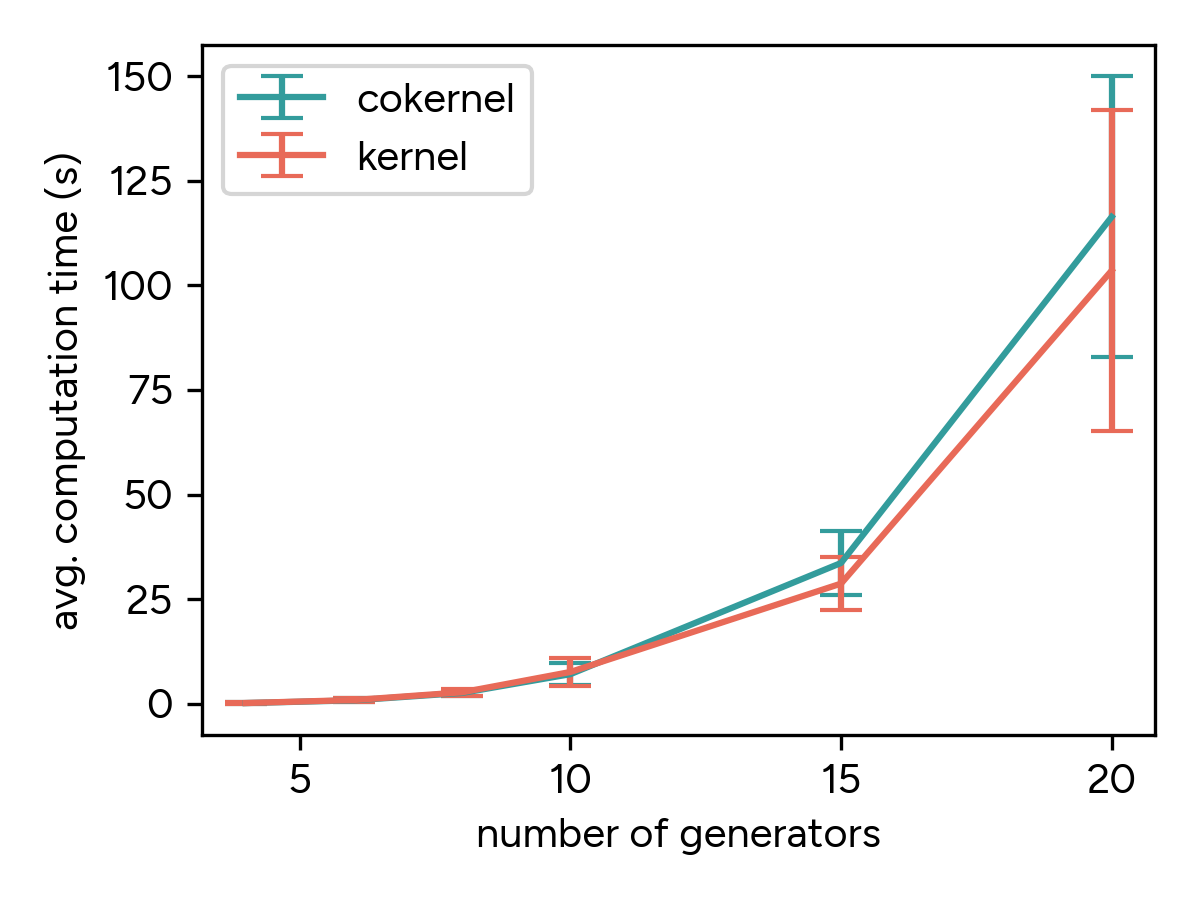
\includegraphics[width=\textwidth]{figs/dev_time.png}
    \caption{Average (of $5$ runs) time to compute relative Betti diagrams with respect to the number of generators.}
    \label{F:dev-time}
  \end{subfigure}
  \hfill
  \begin{subfigure}{.6\textwidth}
    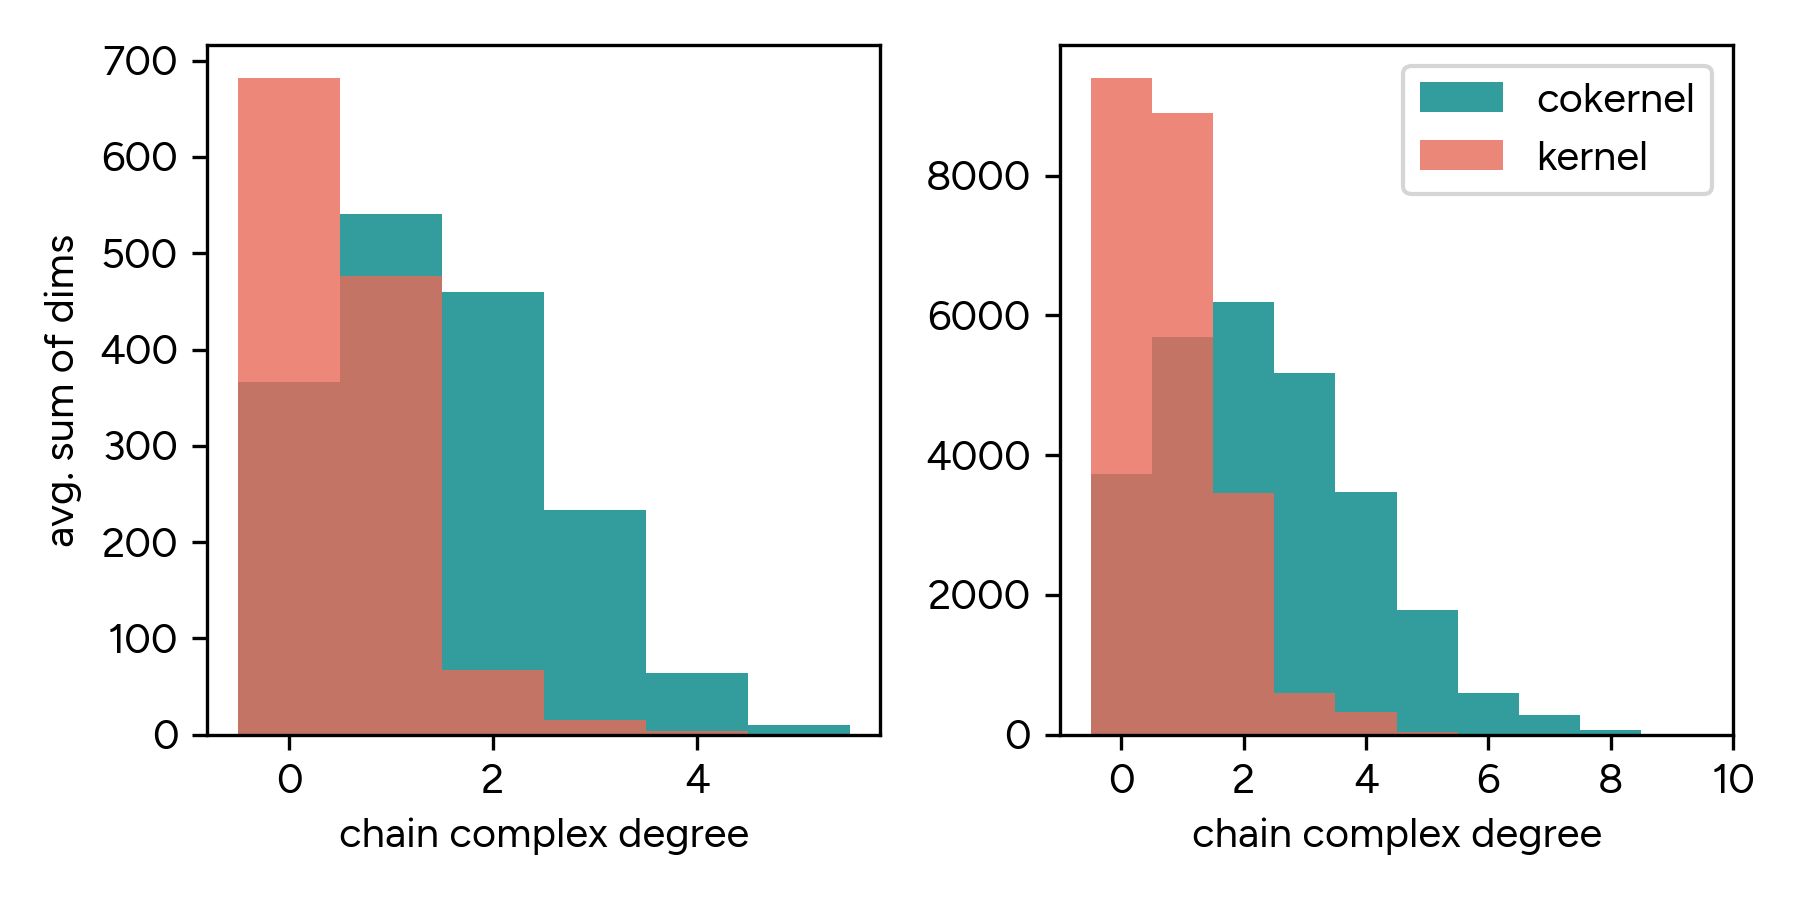
\includegraphics[width=\textwidth]{figs/dev_hist.png}
    \caption{Average (of $10$ runs) sum of dimensions per degree in the Koszul complex of kernels and cokernels for randomly generated persistence modules with $5$ (left) and $10$ (right) generators.}
    \label{F:dev-hist}
  \end{subfigure}
  \caption{Results of the cokernel approach to computing Betti diagrams relative to lower hooks.}
  \label{F:coker-results}
\end{figure}

% \section{Stabilized relative Betti numbers}  % I've kind of avoided defining stabilized ranks

% at IML, with Claudia Landi, Bjørnar Gullikstad Hem, Daniel Tolosa, Berat Geven \ir{surely I don't cite these names, or maybe this result...}

% In \cite{CGRST2024} the authors develop the theory of relative homological algebra for (multiparameter) persistence modules. In particular, given a collection $\mathcal{P}$ of ``simple'' persistence modules, we can define a minimal relative projective resolution of a module $M$ as
% \[
% \cdots \to F_1 \to F_0 \to M \to 0
% \]
% where each $F_i$ is of the form $\bigoplus_{A \in \mathcal{P}} A^{\oplus \beta_i^{\mathcal{P}}M(A)}$, with $\beta_i^{\mathcal{P}} M \colon \mathcal{P} \to \mathbb{N}$ giving the multiplicity of each module $A$ of $\mathcal{P}$ in $F_i$. These multiplicities are the \emph{relative Betti numbers}, and the paper gives a strategy to efficiently compute them for certain collections $\mathcal{P}$, using (local) Koszul complexes. When $\mathcal{P}$ is the collection of free modules, then the relative Betti numbers are exactly the standard Betti numbers; in the notation the $\mathcal{P}$ is omitted.

% Separately, in \cite{GafvertChacholski2021}, the authors show that the hierarchical stabilization of the standard $0^{\text{th}}$ Betti number $\beta_0 M$ is NP-hard to compute, while also giving a strategy for computing them (not so efficiently). We then had two broad research directions:
% \begin{enumerate}
% \item understand the algorithm for computing stabilized $\beta_0$;
% \item understand the stabilized relative $\beta_0$.
% \end{enumerate}
% We focused on the second direction, where we managed to prove the following.

% \paragraph{Result.} If $\{\text{free}\} \subseteq \mathcal{P} \subseteq \{\text{single-source}\}$, where single-source modules are those with a single generator, then $\widehat{\beta_0^{\mathcal{P}} M} \geq \widehat{\beta_0 M}$ for all persistence modules $M$.

% That is, given a fixed noise system, if the collection $\mathcal{P}$ contains all free modules and only contains single-source modules, then the stabilized relative $\beta_0$ is always greater than the stabilized standard $\beta_0$.

% \ir{proof?}

% \section{Dual poset elements for Koszul complexes}

% with Wojciech Chachólski and Marve Grönblad Vesterinen.

% This was a Master's thesis. We define a notion of \term[dual element]{dual elements} for lattices $I$ such that the Betti diagrams of the minimal projective and injective resolutions of a functor over $I$ are dual in some sense.

\section{Space of rank functions}

With Wojiech Chachólski, Andrea Guidolin, Christina Kapatsori, Woojin Kim, Francesca Tombari.

The rank function $\rank V$ of a persistence module $V$ over a poset $I$ (\cref{!D:rank-function}) satisfies the following inequalities. For all chains $a \leq b \leq c \leq d$ in $I$,
\begin{enumerate}
  \item (\term{monotonicity}) $\rank V(a \leq d) \leq \rank V(b \leq c)$, and
  \item (\term{chain-supermodularity}) $\rank V(a \leq d) + \rank V(b \leq c) \leq \rank V(a \leq c) + \rank V(b \leq d)$.
\end{enumerate}
The name \term{chain-supermodularity} comes from \textbf{supermodularity}, a notion studied in probability and order theory \cite{PromislowYoung2005}. Monotone, chain-supermodular functions form a positive convex cone. The broad aim of this project is to study this cone and investigate if we can express rank functions as convex combinations of extremal rays.

As a first step, we study \term{chain-modular} functions, which satisfy the chain-supermodularity condition but with an equality instead of inequality. An interesting question is: which functors have rank functions that are chain-modular? We give some characterizations of the space of chain-modular functions and functors depending on the structure of the underlying poset $I$.
\ir{REVIEW: When $I$ has trivial $H^1$...}

\section{Rank-based noise systems for multiparameter persistence}

With Håvard Bakke Bjerkevik, Andrea Guidolin, and Martina Scolamiero.

For $p \geq n + 1$ and $V \colon \R^n \to \Vect$ an $n$-dimensional persistence module, consider the following integral:
\[
  \| V \|_{p} \coloneq \left( \int_{\vec{x} \leq \vec{y} \in \Omega} p (p - 1)(y_1 - x_1)^{p - n - 1} \rank V(\vec{x} \leq \vec{y}) \right)^{\frac{1}{p}},
\]
where $\Omega \coloneq \{(\vec{x}, \vec{y}) \in (\R^n)^2 \mid \vec{x} \leq \vec{y}\}$ for the product order on $\R^n$.

Following Papers \ref{PC:AGRS2025} and \ref{PC:GRRS2026}, we show the following:

\begin{proposition}
  Let $p \in [n + 1, \infty)$. The $p$-norm on $n$-dimensional persistence modules defines in amplitude. In other words, the $p$-norm defines a noise system.
\end{proposition}

\begin{proof}[Sketch of proof]
  The first, easier short exact sequence axiom (see \cref{!D:noise-system}) comes from [Paper \ref{PC:GRRS2026}, Proposition 4.9], as in the one-dimensional case.

  To prove the second, harder short exact sequence axiom, we proceed as follows. We restrict the rank function of $V$ to lines in $\R^n$ parameterized as $\ell \colon t \mapsto t \vec{a} + \vec{b}$, where $\vec{a} = (1, a_2, \ldots, a_n)$ and $\vec{b} = (0, b_2, \ldots, b_n)$. Then we parameterize our pairs of points $(\vec{x}, \vec{y})$ in $\Omega$ by scalars $s$ and $t$ in $\R$:
  \[
    \vec{x} = s \vec{a} + \vec{b}, \qquad \vec{y} = t \vec{a} + \vec{b}.
  \]
  Then we have the change of parameters
  \begin{equation}
  \label{Eq:reparam}
    \begin{aligned}
      \| V \|_p^p & = \int_{(\vec{x} \leq \vec{y}) \in \Omega} p (p - 1) (y_1 - x_1)^{p - n - 1} \rank V(\vec{x} \leq \vec{y}) \\
      & = \int_{\vec{a} \geq 0} \int_{\vec{b} \in \R^n} \int_{s = -\infty}^{+\infty} \int_{t = s}^{+\infty} p (p - 1) (t - s)^{p - 2} \rank V(\vec{p}, \vec{q}) \text{d}t \text{d}s \text{d}\vec{b} \text{d}\vec{a},
    \end{aligned}
  \end{equation}
  where the proof relies on the computation of the Jacobian of the change of parameters:
  \[
    J_\varphi = \bordermatrix{%
    & s & t & a_2 & b_2 & a_3 & b_3 & \cdots \cr
    p_1 & 1 & 0 \cr
    q_1 & 0 & 1 \cr
    p_2 & a_2 & 0 & s & 1 \cr
    q_2 & 0 & a_2 & t & 1 \cr
    p_3 & a_3 & 0 &&& s & 1 \cr
    q_3 & 0 & a_3 &&& t & 1 \cr
    \vdots & \vdots & \vdots &&&&& \ddots
    }
  \]
  In particular, we have $|\det J_\varphi| = (t - s)^{n - 1}$.

  For a given line $\ell \colon t \mapsto t \vec{a} + \vec{b}$, we apply the result that the $p$-norm gives a noise system in the one-dimensional case. In particular, given a short exact sequence $0 \to U \to V \to W \to 0$ of $n$-dimensional persistence modules, we use the characterization of $p$-norms as integrals of the rank function [Paper \ref{PC:GRRS2026}, Proposition 4.7] to obtain the following triangular inequality:
  \begin{align*}
    & \left(\int_{s = -\infty}^{+\infty} \int_{t = s}^{+\infty} p (p - 1) (t - s)^{p - 2} \rank V(\vec{x} \leq \vec{y}) \text{d}t \text{d}s\right)^{\frac{1}{p}} \\
    & \leq \left(\int_{s = -\infty}^{+\infty} \int_{t = s}^{+\infty} p (p - 1) (t - s)^{p - 2} \rank U(\vec{x} \leq \vec{y}) \text{d}t \text{d}s\right)^{\frac{1}{p}} \\
    & \hspace{2em} + \left(\int_{s = -\infty}^{+\infty} \int_{t = s}^{+\infty} p (p - 1) (t - s)^{p - 2} \rank W(\vec{x} \leq \vec{y}) \text{d}t \text{d}s\right)^{\frac{1}{p}}.
  \end{align*}
  Let
  \[
    f(\vec{a},\vec{b}) \coloneq (\int_{-\infty}^\infty \int_s^\infty p (p - 1) (t-s)^{p - 2} \rank U(\vec{x} \leq \vec{y}) dt ds)^{\frac 1p},
  \]
  and define $g$ and $h$ similarly. Then the previous equations rewrites as $f \leq g + h$.

  We can apply Minkowski's inequality, which states that $(\int (f + g)^p)^{\frac 1p} \leq (\int f^p)^{\frac 1p} + (\int g^p)^{\frac 1p}$ holds for $1 \leq p < \infty$. We get
  \[
    (\int_{\vec{a}} \int_{\vec{b}} f(\vec{a}, \vec{b})^p d\vec{b} d\vec{a})^{\frac{1}{p}} \leq (\int_{\vec{a}} \int_{\vec{b}} g(\vec{a}, \vec{b})^p d\vec{b} d\vec{a})^{\frac{1}{p}} + (\int_{\vec{a}} \int_{\vec{b}} h(\vec{a}, \vec{b})^p d\vec{b} d\vec{a})^{\frac{1}{p}}.
  \]
  By \eqref{Eq:reparam}, this exactly says that
  \[
    \| V \|_p \leq \| U \|_p + \| W \|_p,
  \]
  and this is the hard axiom of noise systems.
\end{proof}

% \section{Matching costs}

% $\| \mu_1 \bullet \mu_2 \|_p \leq \| \mu_1 \|_p \| \mu_2 \|_p$ ?

\section{\texorpdfstring{$p$}{p}-norms of extensions}

This is the content of Hugo Åkesson's Masters thesis \cite{Åkesson2023}, which I co-supervised with Wojciech Chachólski.

Let $V$ and $W$ be persistence modules. An \term[extension]{extension of $V$ by $W$} is a persistence module $E$ that fits into a short exact sequence
\[
  0 \to W \to E \to V \to 0.
\]
We denote by $\Ext(V, W)$ the collection of extensions up to isomorphism (a morphism of extensions is one that commutes with the maps from $W$ and to $V$), and it turns out that this collection forms a vector space.
The question that Åkesson studied is: what is the maximal $p$-norm of an extension? We have results if $W$ is a single bar:

\begin{theorem}[{\cite[Theorem 3.1]{Åkesson2023}}]
\label{T:antichain-extensions-1}
  Let $V$ be a tame persistence module and $[a, b)$ an interval of $\R$. Write
  \[
    F^{ab}(V) \coloneq \{(c, d) \in \cc{D}(V) \mid a < c \leq b < d\}.
  \]
  Then there exists explicitly constructed bijection
  \[
    \psi \colon \{ \text{antichains in } F^ab(V) \} \cong \barcode(\Ext(\K_{[a, b)}, V)),
  \]
  where antichains are defined in [Paper \ref{PC:CGRST2024}, \textsection 4.6] and $\barcode(-)$ is the set of barcodes of elements of the argument.
\end{theorem}

Moreover, we can equip antichains with a partial order $\preceq$ (see again [Paper \ref{PC:CGRST2024}, \textsection 4.6]) such that the following result holds.

\begin{theorem}[{\cite[Theorem 3.2]{Åkesson2023}}]
\label{T:antichain-extension-2}
  We use the notations of \cref{T:antichain-extensions-1} and fix $p \in [1, \infty]$. The function $A \mapsto \| \psi(A) \|_p$ from antichains in $F^{ab}(V)$ to $p$-norms is monotone. In other words, for antichains $A$ and $B$ in $F^{ab}$,
  \[
    A \preceq B \quad \Rightarrow \quad \| \psi(A) \|_p \leq \| \psi(B) \|_p.
  \]
\end{theorem}

Notably, the poset of antichains of $F^{ab}$ has a greatest element, the antichain of maximal elements of $F^{ab}$. By \cref{T:antichain-extension-2}, the bijection $\psi$ sends this antichain to the extension barcode with the greatest $p$-norm.

When $W$ is arbitrary, Åkesson provides a recursive formula \cite[Theorem 4.1]{Åkesson2023}: if $W = W_1 \oplus W_2$ with $\Ext(W_1, W_2) = 0$ (this is always possible), then
\begin{equation}
\label{Eq:recursive-extension}
  \barcode(\Ext(W, V)) = \bigcup_{B \in \barcode(\Ext(W_2, V))} \barcode(\Ext(W_1, \cc{V}(B))),
\end{equation}
where $\cc{V}(B)$ is a persistence module with barcode $B$. This gives an iterative strategy for computing $\barcode(\Ext(W, V))$: sort the bars of $W$ compatibly with the product order on the start- and endpoints, set $W_2$ equal to the first bar and $W_1$ to the sum of the rest: by construction, we get $\Ext(W_1, W_2) = 0$.

It is still an open problem to determine the extension with largest $p$-norm. This is useful, for example, in the study of the noise system axioms for $p$-norms.

\section{Pair degree}

Following discussions with Emil Horobeț.

In Papers \ref{PC:GLRS2025} and \ref{PC:Ren2026}, we defined notions of algebraic critical points, and bounded their number. The number of algebraic critical points, in the complex setting, could define a new numerical invariant that generalizes the Euclidean distance degree and the bottleneck degree. Here we sketch its definition:

\begin{definition}
  Let $X$ and $Y$ be complete intersections defined by polynomials $\vec{p}$ and $\vec{q}$, respectively. We define the \term[pair degree]{pair degree of $X$ and $Y$} to be the cardinality of the set $C_k(\vec{p}, \vec{q})$ of algebraic critical points of the distance function $\dist_Y\big|_X$ (see Paper \ref{PC:Ren2026}, Definition 3.3.2).
\end{definition}

\ir{REVIEW: Say a bit more}